% Source: AESP_466_ClassWork/Supplements/Notes/latex/6.2.5/6.2.5.tex

\documentclass[border=4pt]{standalone}
\usepackage{amsmath,amssymb,amsthm}
\usepackage{graphicx}
\usepackage{tikz}
\usepackage{xcolor}
\usetikzlibrary{arrows.meta,calc,positioning,decorations.markings,patterns,shapes.geometric,angles,quotes}

\definecolor{Garnet}{HTML}{73000A}
\definecolor{USC_Rose}{HTML}{CC2E40}
\definecolor{USC_Blue}{HTML}{466A9F}
\definecolor{USC_Slate}{HTML}{1F414D}
\definecolor{USC_Olive}{HTML}{65780B}
\definecolor{USC_Lime}{HTML}{CED318}
\definecolor{USC_Gold}{HTML}{A49137}
\definecolor{USC_Black90}{HTML}{565556}
\definecolor{USC_Black10}{HTML}{ECECEC}

\newcommand{\vect}[1]{\mathbf{#1}}
\newcommand{\mat}[1]{\mathbf{#1}}
\newcommand{\uvec}[1]{\hat{\mathbf{#1}}}
\newcommand{\transpose}{^{\mkern-1.5mu\mathsf{T}}}
\newcommand{\inv}{^{-1}}
\newcommand{\deriv}[2]{\frac{d #1}{d #2}}
\newcommand{\pderiv}[2]{\frac{\partial #1}{\partial #2}}

\begin{document}
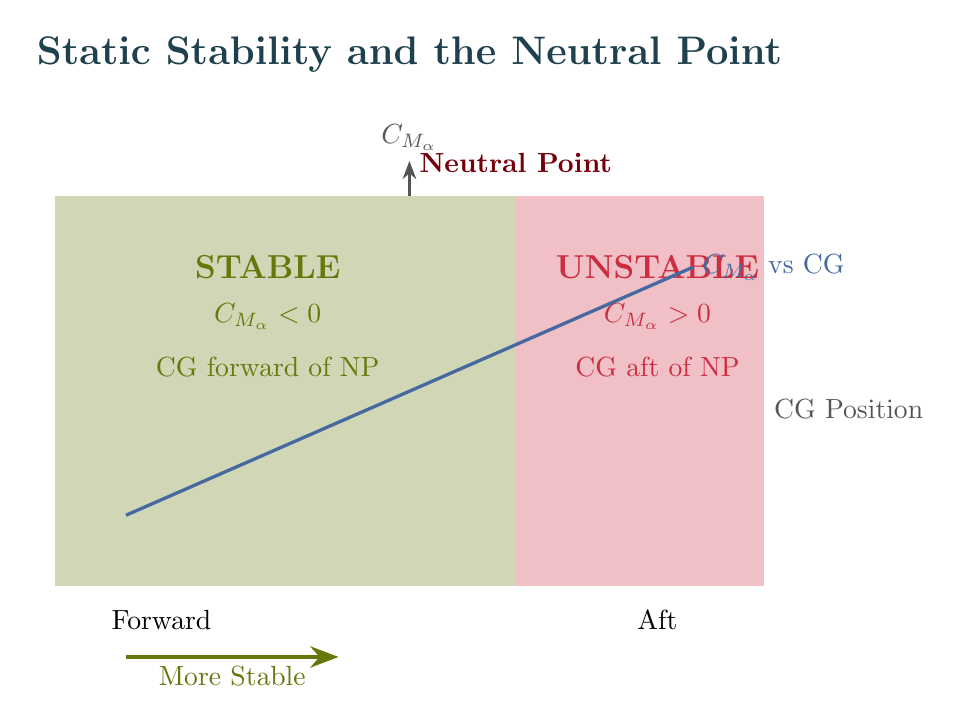
\begin{tikzpicture}[>=Stealth, scale=0.9]
    % Title
    \node[font=\Large\bfseries, USC_Slate] at (0,5) {Static Stability and the Neutral Point};

    % Horizontal axis (CG position)
    \draw[->, thick, USC_Black90] (-5,0) -- (5,0) node[right] {CG Position};

    % Vertical axis (stability)
    \draw[->, thick, USC_Black90] (0,-2.5) -- (0,3.5) node[above] {$C_{M_\alpha}$};

    % Neutral point marker
    \draw[ultra thick, Garnet] (1.5,-2.5) -- (1.5,3);
    \node[Garnet, above] at (1.5,3.2) {\textbf{Neutral Point}};
    \fill[Garnet] (1.5,0) circle (0.12);

    % Stability regions
    \fill[USC_Olive!30] (-5,-2.5) rectangle (1.5,3);
    \fill[USC_Rose!30] (1.5,-2.5) rectangle (5,3);

    % Labels for regions
    \node[USC_Olive, font=\large\bfseries] at (-2,2) {STABLE};
    \node[USC_Olive] at (-2,1.3) {$C_{M_\alpha} < 0$};
    \node[USC_Olive] at (-2,0.6) {CG forward of NP};

    \node[USC_Rose, font=\large\bfseries] at (3.5,2) {UNSTABLE};
    \node[USC_Rose] at (3.5,1.3) {$C_{M_\alpha} > 0$};
    \node[USC_Rose] at (3.5,0.6) {CG aft of NP};

    % Slope indication line
    \draw[very thick, USC_Blue] (-4,-1.5) -- (4,2);
    \node[USC_Blue, right] at (4,2) {$C_{M_\alpha}$ vs CG};

    % Forward/Aft labels
    \node[below] at (-3.5,-2.7) {Forward};
    \node[below] at (3.5,-2.7) {Aft};

    % Arrow showing preferred direction
    \draw[->, ultra thick, USC_Olive] (-4,-3.5) -- (-1,-3.5);
    \node[USC_Olive, below] at (-2.5,-3.5) {More Stable};

\end{tikzpicture}
\end{document}
